\documentclass{beamer}
\usepackage{minted}
\usepackage{transparent}
\usetheme{Boadilla}
\usepackage[ddmmyyyy]{datetime}
\usecolortheme{whale}
\setbeamercovered{transparent}
\setbeamertemplate{caption}{\raggedright\insertcaption\par}
\newcommand\Fontvi{\fontsize{9.5}{7.2}\selectfont}
\usepackage[T1]{fontenc}

\usepackage{color}
\usepackage{listings}
\lstset{language=Go,
  basicstyle=\ttfamily\scriptsize,
  keywordstyle=\color{blue}\ttfamily,
  stringstyle=\color{red}\ttfamily,
  commentstyle=\color{green}\ttfamily}


\begin{document}

\title[Golang e modelli di concorrenza]{Golang e modelli di concorrenza}
\author{Leonardo Gonfiantini}
\date{27 Ottobre 2022}
\begin{frame}
\centerline{
\includegraphics[width=2cm,height=2cm,keepaspectratio]{logo-unige-pulito.png}}
  \titlepage
  \centerline{Relatore: Delzanno Giorgio}
\end{frame}

\begin{frame}
  \frametitle{Golang}
  \begin{columns}
    \begin{column}{0.6\textwidth}
      \begin{itemize}
        \item linguaggio compilato e tipato staticamente, creato da Google
        \item sintatticamente simile al C ma con: \begin{itemize}
            \item memory safety
            \item garbage collection
            \item structural typing
            \item CSP-style concurreny
        \end{itemize}
        \pause
        \item alte prestazioni per il networking e multiprocessing
        \item open-source
      \end{itemize}
    \end{column}
    \begin{column}{0.4\textwidth}
      \centerline{
\includegraphics[width=5cm,height=5cm,keepaspectratio]{go-mascotte.jpg}}
    \end{column}
  \end{columns}
\end{frame}
\begin{frame}{CSP - Communicating sequential processes}

\centering
\textit{“Don’t communicate in the form of shared memory. Instead, share memory
through communication.”}

\vspace{1cm}

Generalmente nei linguaggi come C, C++ e Java la comunicazione tra thread avviene utilizzando la memoria condivisa, questo Go lo puo fare, ma puo anche utilizzare i modelli di concorrenza del CSP tramite l'utilizzo dei canali.
\end{frame}

\begin{frame}{Channel}

\centerline{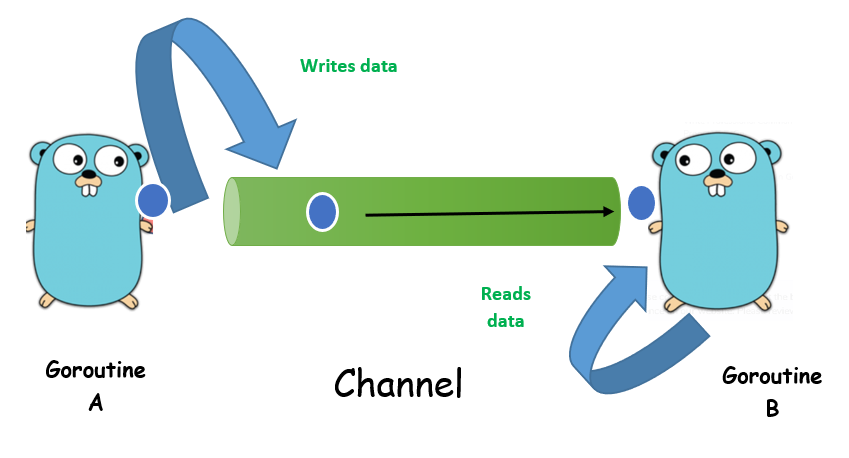
\includegraphics[width=8cm,height=5cm,keepaspectratio]{goroutine-channel.png}}

I canali funzionano come dei tubi alla quale diversi thread (\textbf{goroutine}), possono collegarsi, la comunicazione e' bidirezionale per default, il che significa che possiamo ricevere e inviare messaggi dallo stesso canale.

\vspace{0.50cm}

\pause

Questo permette alle goroutine di sincronizzarsi non utilizzando lock o condition variable.
    
\end{frame}

\begin{frame}[fragile]{Channel - dichiarazione}
  \begin{columns}
    \begin{column}{0.4\textwidth}
    \begin{lstlisting}
    
    //unbuffered channel
    ch := make(ch int) //init
    ch <- 42 //inviamo 42
    
    n := <- ch 
    //riceviamo dal canale 42
    
    //nel caso di buffered channel
    ch := make(ch int, 10)
    ch <- 42 ch <- 12 ch <- 3
    
    fmt.Println(<- ch, <- ch, <- ch)
    //output = 42 12 3
    
    \end{lstlisting}
   \end{column}
   \begin{column}{0.8\textwidth}
     
    \centerline{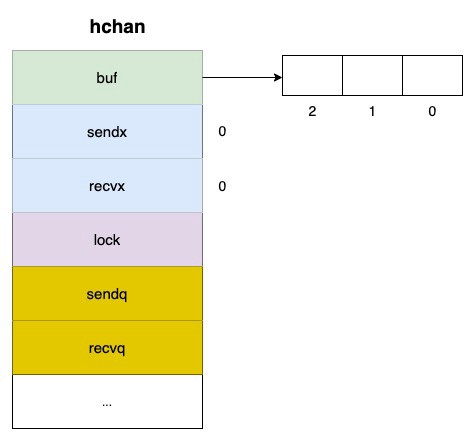
\includegraphics[width=8cm,height=5cm,keepaspectratio]{channel-struct.jpeg}}
    
   \end{column}
  \end{columns}
\end{frame}
\begin{frame}[fragile]{Channel - channel vs mutex}

\begin{columns}
    \begin{column}{0.5\textwidth}
            \centerline{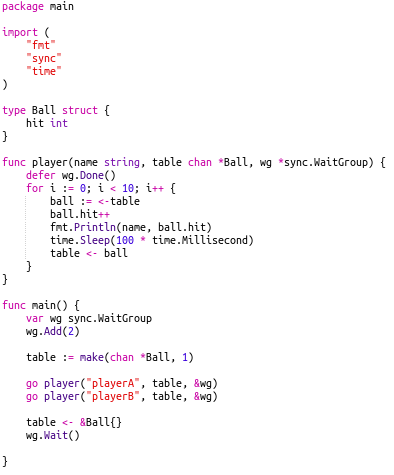
\includegraphics[width=10cm,height=7.5cm,keepaspectratio]{screen1.png}}
    \end{column}
    
    \begin{column}{0.5\textwidth}
            \centerline{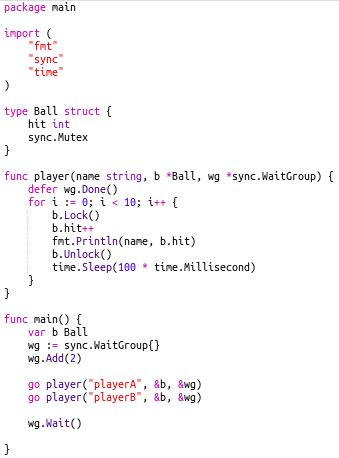
\includegraphics[width=10cm,height=7.5cm,keepaspectratio]{screen2.png}}
    \end{column}
           
\end{columns}
    
\end{frame}

\begin{frame}{Channel - pro e contro}
    
    \begin{center}
    Mutex e channel sono strumenti diversi, i mutex sono utili per accedere ad una risorsa in modo sequenziale e performante, i channel per gestire la comunicazione tra diverse goroutine.
    \end{center}
    
    \vspace{0.7cm}
    
    Quando usare i channel?
    \pause
    \begin{itemize}
        \item passare la ownership del dato
        \item distribuire unita di lavoro (\textbf{worker})
        \item comunicare risultati asincroni
    \end{itemize}
    
\end{frame}

\begin{frame}{Worker pattern}

\centerline{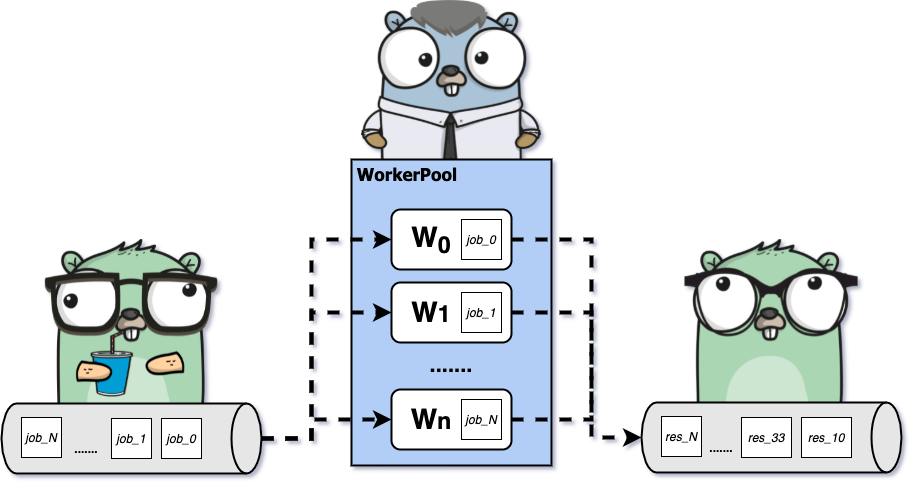
\includegraphics[width=6cm,height=6cm, keepaspectratio]{worker-pool.png}}

\vspace{1cm}

\centering La worker pool viene utilizzata per assegnare un numero n di Tasks ad un numero m di Workers. Le task dovranno stare in una queue, quando un Worker finisce una task controlla se nella queue sono presenti altre task, se si, procedera con la nuova task altrimenti aspettera. 
\end{frame}

\begin{frame}{Worker pattern - implementazione}
    
    \begin{columns}
    \begin{column}{0.6\textwidth}
        \centerline{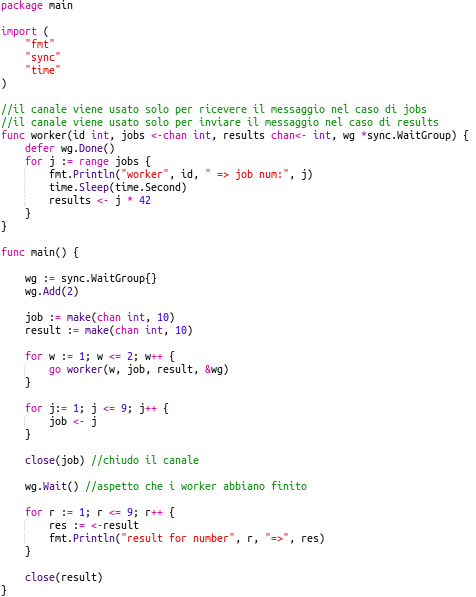
\includegraphics[width=8.5cm,height=7.5cm, keepaspectratio]{screen3.png}}
    \end{column}
    
    \begin{column}{0.4\textwidth}
                \centerline{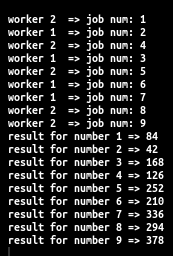
\includegraphics[width=6cm,height=5cm, keepaspectratio]{screen4.png}}
    \end{column}
    
    \end{columns}
\end{frame}

\begin{frame}{Pooling pattern}
\centering Il Pool pattern mostra come utilizzare un canale per creare una pool di risorse condivise che possono essere utilizzate da diverse goroutine singolarmente. \newline
Quando una goroutine ha bisogno di una risorsa dalla pool, viene acquisita,
usata, e ritornata alla pool.
\end{frame}


\begin{frame}{Pooling pattern - implementazione}
    
\end{frame}

\begin{frame}{Riferimenti}
    
\end{frame}

\end{document}